\subsection{JaCaMo}

JaCaMo è un framework per la programmazione orientata agli agenti che combina tre tecnologie già affermate e sviluppate da diversi anni.

\medskip

Un sistema multi-agente JaCaMo o, equivalentemente, un sistema software programmato con JaCaMo è definito da un'organizzazione Moise di agenti BDI autonomi basati su concetti come ruoli, gruppi, missione e schemi, implementati tramite Jason, che lavorano in ambienti condivisi distribuiti basati su artefatti, programmati in CArtAgO.

\medskip

Ognuna delle tre tecnologie indipendenti che compongono il framework ha il proprio set di astrazioni, modelli di programmazione e meta-modelli di riferimento, per questo motivo in JaCaMo è stato realizzato un meta-modello globale, con l'obiettivo di definire le dipendenze, connessioni, mapping concettuali e le sinergie tra le differenti astrazioni rese disponibili da ogni livello \cite{BOISSIER2013747}.

\begin{figure}[H]
\centering
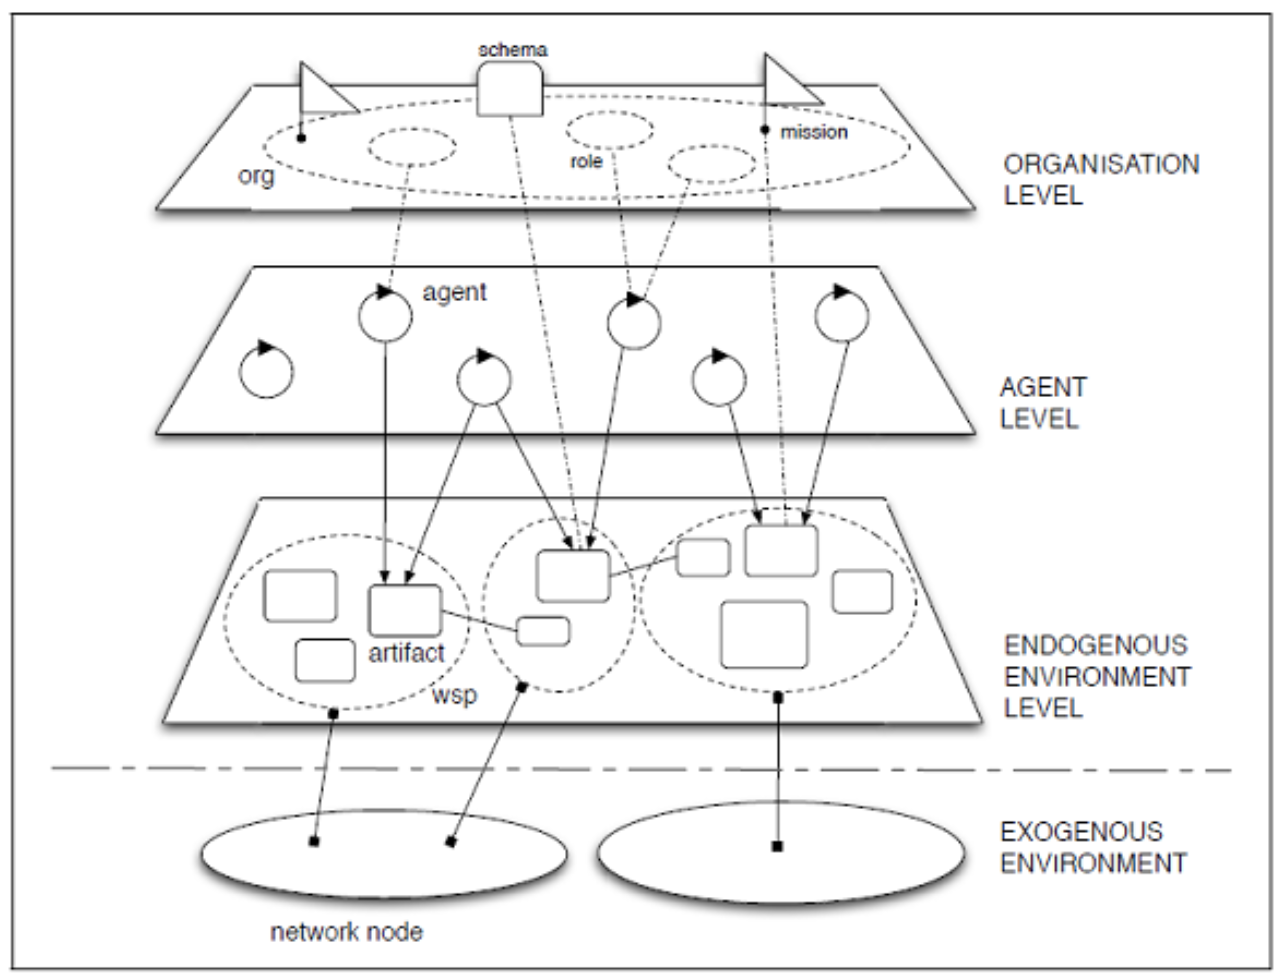
\includegraphics[width=\textwidth]{figures/JaCaMo_levels.png}
\caption{Livelli che compongono il framework JaCaMo \cite{BOISSIER2013747}}
\label{livelli_jacamo}
\end{figure}

\subsubsection{Jason} \label{jason}

Jason è un interprete di AgentSpeak che implementa la semantica operazionale del linguaggio e fornisce una piattaforma di sviluppo per Sistemi Multi-Agente, con molte funzionalità personalizzabili dall'utente.

\medskip

Le astrazioni appartenenti alla dimensione degli agenti, correlate al meta-modello Jason, sono principalmente ispirate all'architettura BDI sulla quale Jason è radicato. Quindi un agente è un'entità composta da un insieme di "beliefs", che rappresenta lo stato corrente e la conoscenza dell'agente sull'ambiente in cui si trova, una serie di "goals", che corrispondono a compiti che l'agente deve perseguire e una serie di "plans" ossia sequenze di azioni (external action or internal action), innescate da eventi, che gli agenti possono comporre, istanziare ed eseguire dinamicamente per compiere i "goals" \cite{jason-book}.

\subsubsection{CArtAgo}
Per quanto riguarda l'ambiente, ciascuna istanza dell'ambiente CArtAgO\footnote{Common ARTifact infrastructure for AGents Open environments} è composta da una o più entità workspace. Ogni workspace è formato da un insieme di artefatti, che forniscono un insieme di operazioni e proprietà osservabili, definendo anche l'interfaccia di utilizzo degli artefatti. L'esecuzione dell'operazione potrebbe generare aggiornamenti delle proprietà osservabili e degli eventi osservabili specifici. L'ultima entità relativa all'ambiente è il “manual”, un'entità utilizzata per descrivere le funzionalità fornite da un artefatto.
Cartago è basato sul meta-modello A\&A (Agents \& Artifacts), che definisce gli agenti come entità computazionali che compiono qualche tipo di attività che mira a uno scopo e gli artefatti come risorse e strumenti costruiti dinamicamente, usati e manipolati dagli agenti per supportare/realizzare le loro attività \cite{cartago}.

\smallskip

\paragraph{Artefatto}
L'artefatto è un'entità reattiva, non autonoma, stateful, riutilizzabile, controllabile ed osservabile. Modellano strumenti, risorse e porzioni di ambiente agendo da strumenti mediatori di azioni e interazioni sociali tra partecipanti individuali e lo stesso ambiente \cite{Omicini2008}.

\begin{figure}[H]
\centering
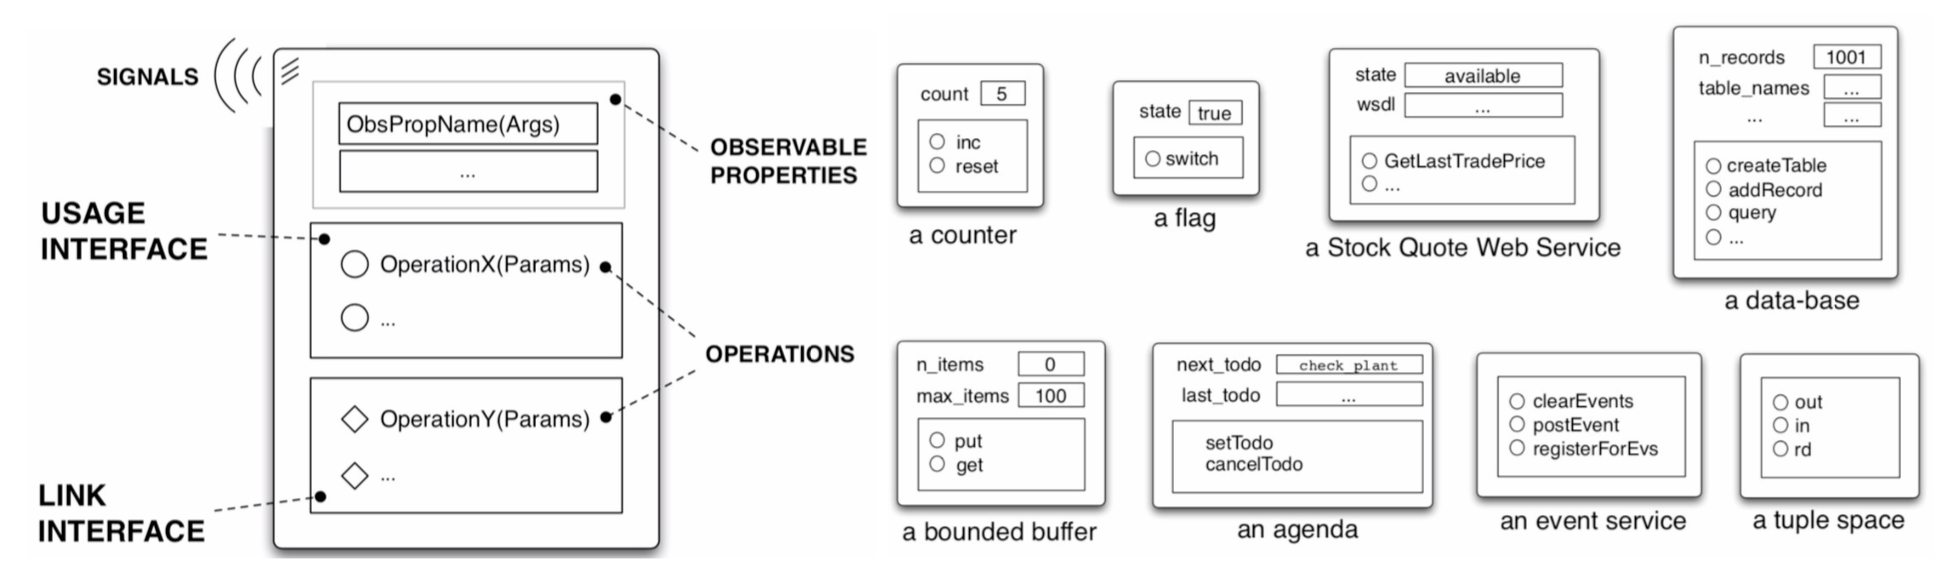
\includegraphics[width=\linewidth]{figures/Artifact_structure_example.png}
\caption{Struttura artefatto con relativi esempi}
\end{figure}

La modalità di interazione tra artefatto ed agente viene riepilogato nell'immagine sottostante.

\begin{figure}[H]
\centering
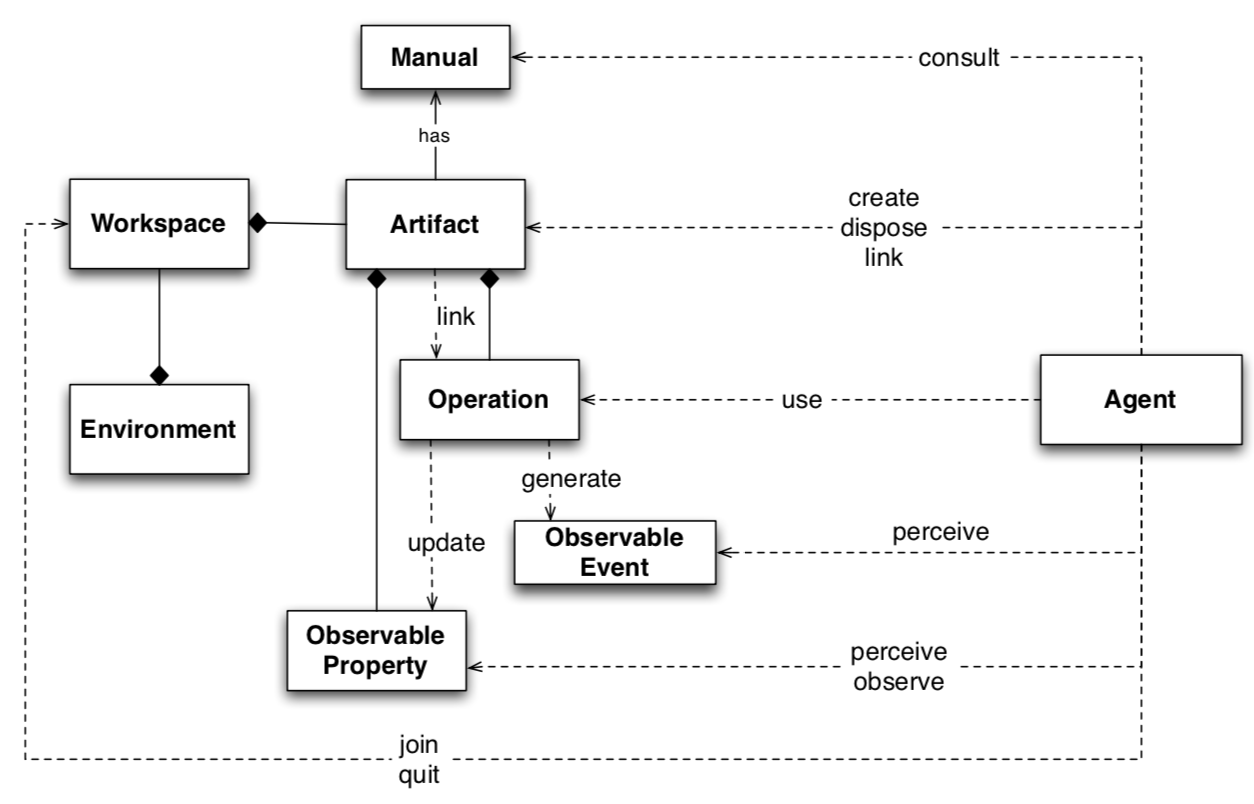
\includegraphics[width=\linewidth]{figures/Artifact_Agent_interaction.png}
\caption{Interazione tra agente ed artefatto}
\end{figure}

\subsubsection{Moise}
Moise è un meta-modello organizzativo per MAS basato sulle nozioni di ruoli, gruppi e missioni. Abilita un MAS ad avere specifiche esplicite per la sua organizzazione. Queste specifiche sono usate sia dagli agenti per ragioni inerenti la loro organizzazione, sia da una piattaforma organizzativa che si assicuri che gli agenti seguano le specifiche.

Moise permette di definire una gerarchia di ruoli con autorizzazioni e missioni, da assegnare agli agenti. Questo permette ai sistemi con un'organizzazione forte, di guadagnare proprietà di apertura (essenzialmente, la proprietà di lavorare con un numero e una diversità di componenti che non è imposta una volta per tutte) e adattamento.
